\documentclass{beamer}

\usetheme{Madrid}
\usecolortheme{default}

\title[Sentiment Analysis]{Neural Approaches to Sentiment Classification of Instagram Comments}
\subtitle{A Pattern Recognition Study in Three Emotional Categories}
\author{Mandira Majhi \and Manopriya Pal \and Bishwayan Ghosh \and Baidurya Bhattacharyya}
\institute{Indian Statistical Institute}
\date{\today}

\begin{document}

% ------------------------------------------------------------
\begin{frame}
    \titlepage
\end{frame}

% ------------------------------------------------------------
\begin{frame}{Introduction}
    \begin{itemize}
        \item Instagram comments are short, noisy, and informal.
        \item Goal: classify 1333 comments into 3 sentiment categories.
        \item Challenges: slang, emojis, sarcasm, sparse lexical signals.
    \end{itemize}
\end{frame}

% ------------------------------------------------------------
\begin{frame}{Dataset Overview}
    \begin{itemize}
        \item 1333 manually labelled comments.
        \item Each row includes context, raw comment, sentiment label.
    \end{itemize}

    \begin{center}
        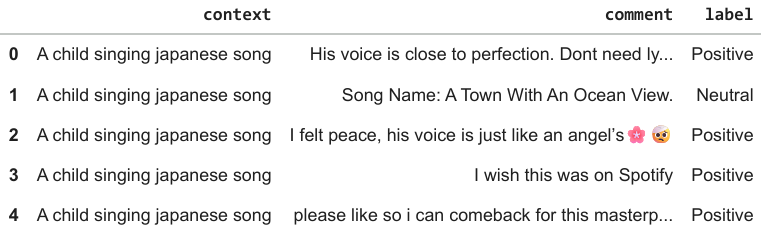
\includegraphics[width=0.55\linewidth]{dataset.png}
    \end{center}
\end{frame}

% ------------------------------------------------------------
\begin{frame}{Label Distribution and Comment Length}
    \begin{center}
        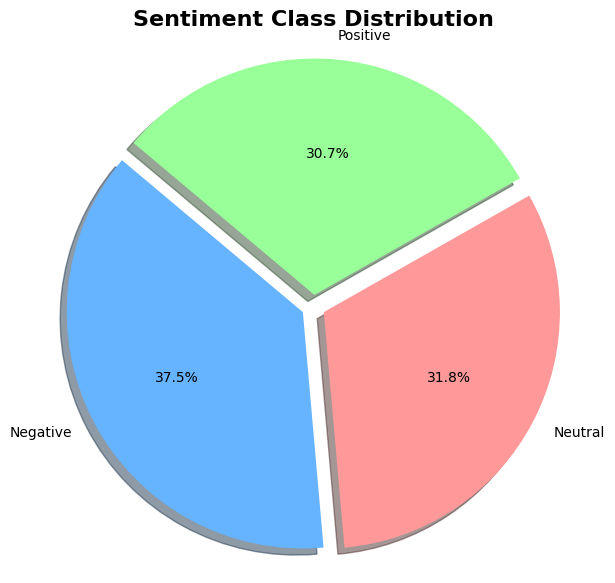
\includegraphics[width=0.3\linewidth]{class-dist-pie.png}
        
        \vspace{0.4cm}
        
        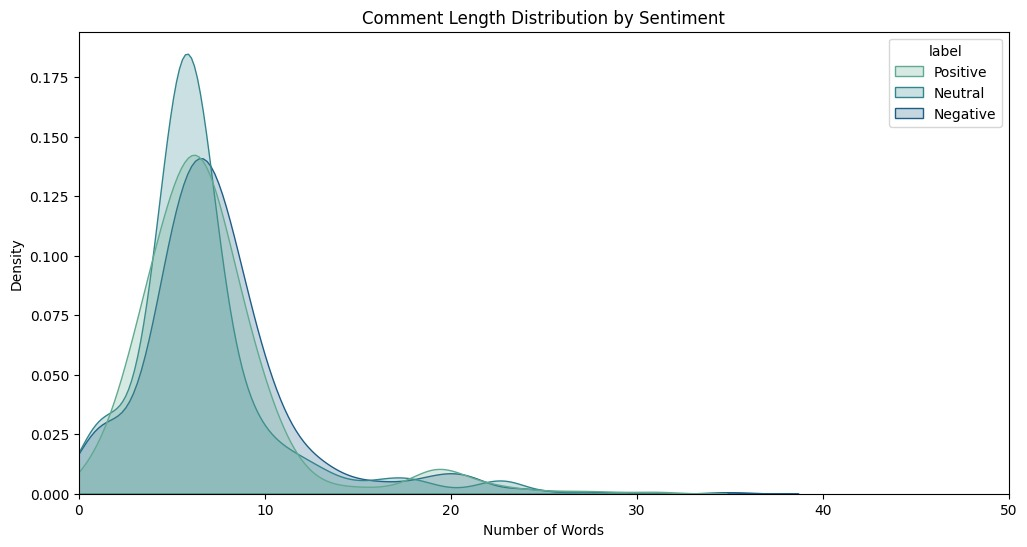
\includegraphics[width=0.6\linewidth]{comment-length.jpg}
    \end{center}
\end{frame}

\begin{frame}{Wordclouds}

\begin{center}
    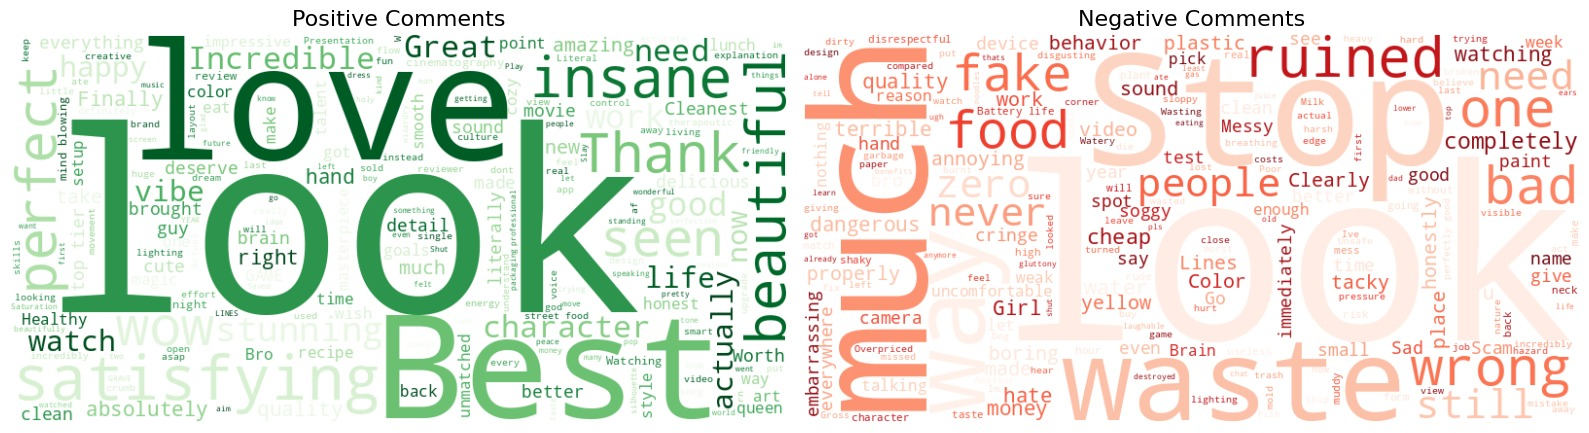
\includegraphics[width=\linewidth]{image.png}
\end{center}
    
\end{frame}

% ------------------------------------------------------------
\begin{frame}{Preprocessing}
    \begin{itemize}
        \item Lowercasing, removing URLs/hashtags/mentions/emojis.
        \item Punctuation stripping.
        \item Tokenisation, stopword removal, lemmatisation.
        \item CountVectorizer (5000 features) for classical models.
    \end{itemize}
\end{frame}

% ------------------------------------------------------------
\begin{frame}{Models Used}
    \begin{itemize}
        \item Logistic Regression
        \item Linear Support Vector Machine
        \item Multinomial Naive Bayes
        \item XGBoost
        \item DistilBERT (fine-tuned transformer)
    \end{itemize}
\end{frame}

% ------------------------------------------------------------
\begin{frame}{Confusion Matrices (All Models)}
    \begin{center}
        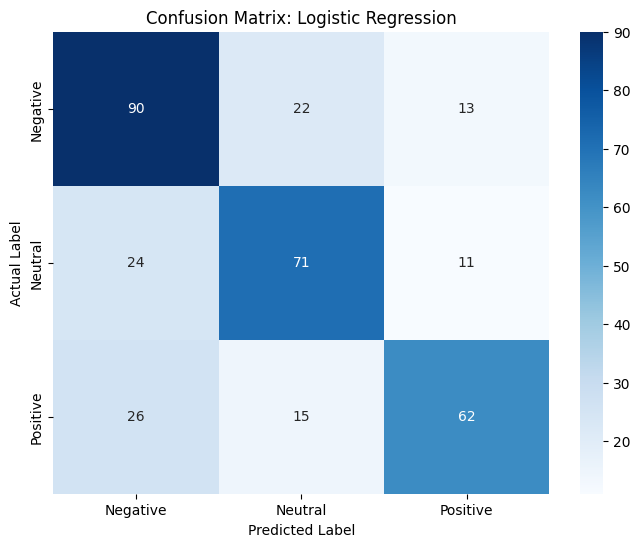
\includegraphics[width=0.25\linewidth]{conf-logistic.png}
        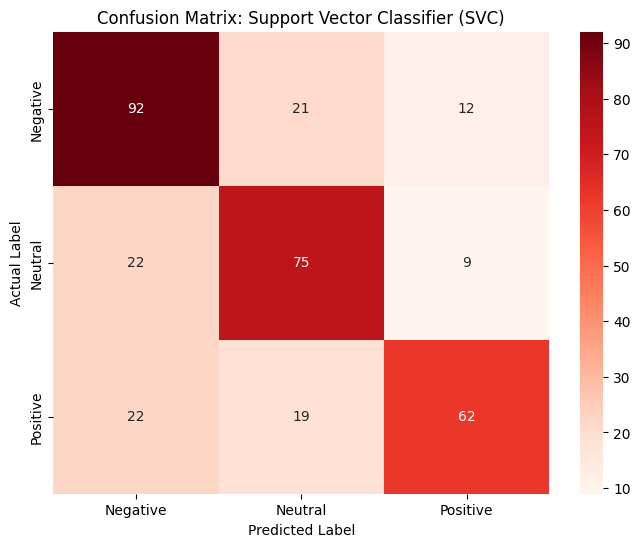
\includegraphics[width=0.25\linewidth]{conf-svc.png}

        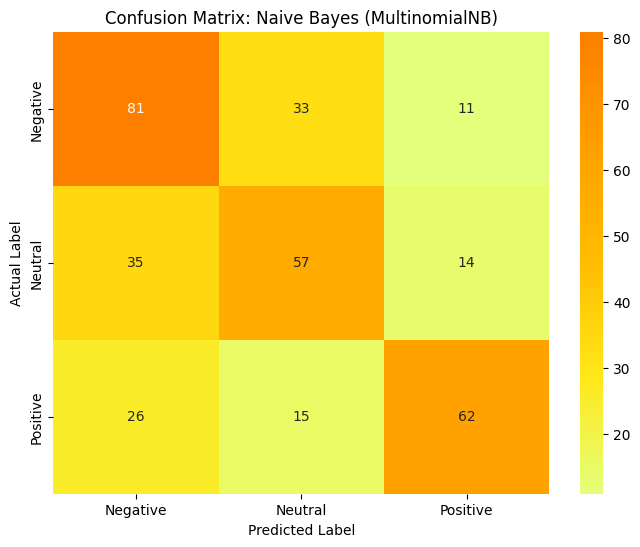
\includegraphics[width=0.25\linewidth]{conf-mult.png}
        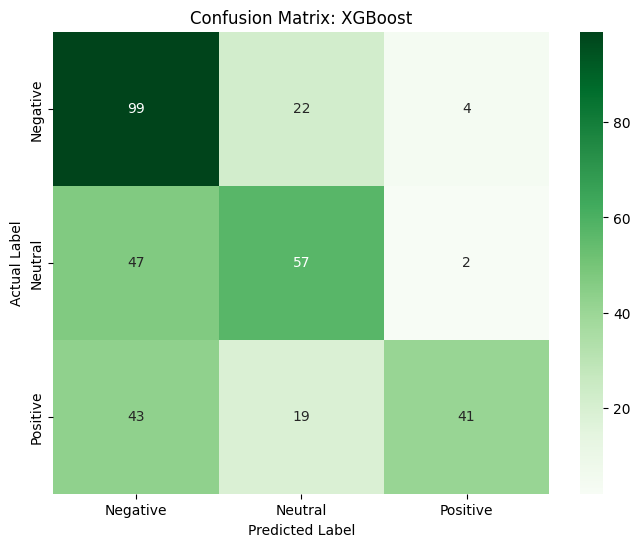
\includegraphics[width=0.25\linewidth]{conf-xgb.png}

        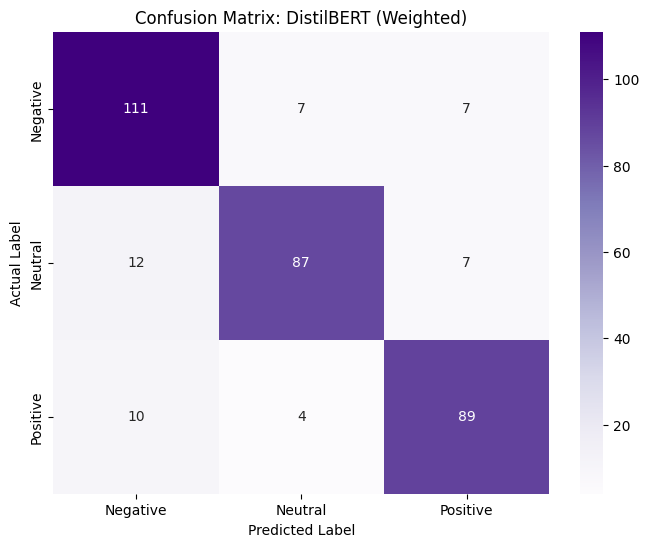
\includegraphics[width=0.25\linewidth]{conf-distil.png}
    \end{center}
\end{frame}

% ------------------------------------------------------------
\begin{frame}{Classwise Recalls}
    \begin{center}
        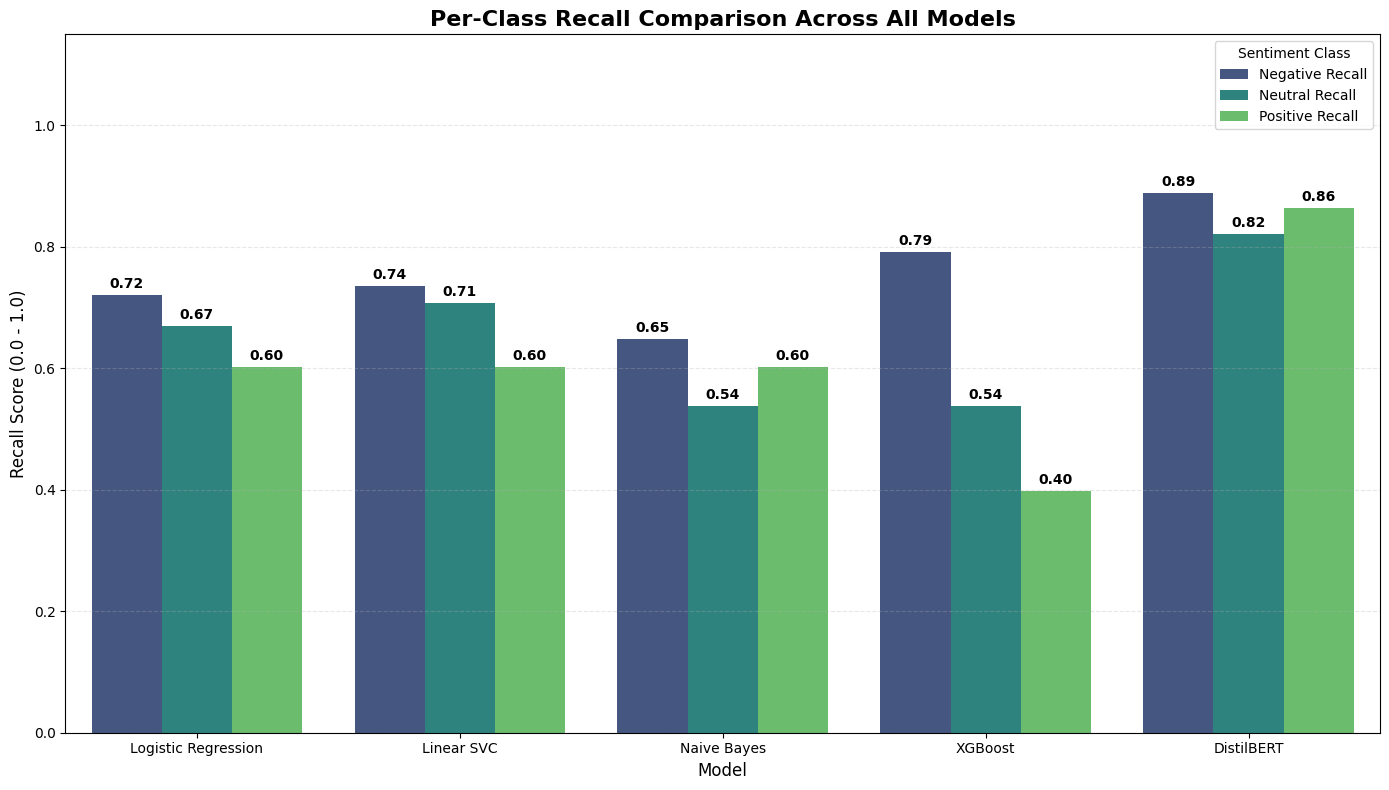
\includegraphics[width=0.9\linewidth]{compare-recall.png}
    \end{center}
\end{frame}

% ------------------------------------------------------------
\begin{frame}{F1 Score Comparison}
    \begin{center}
        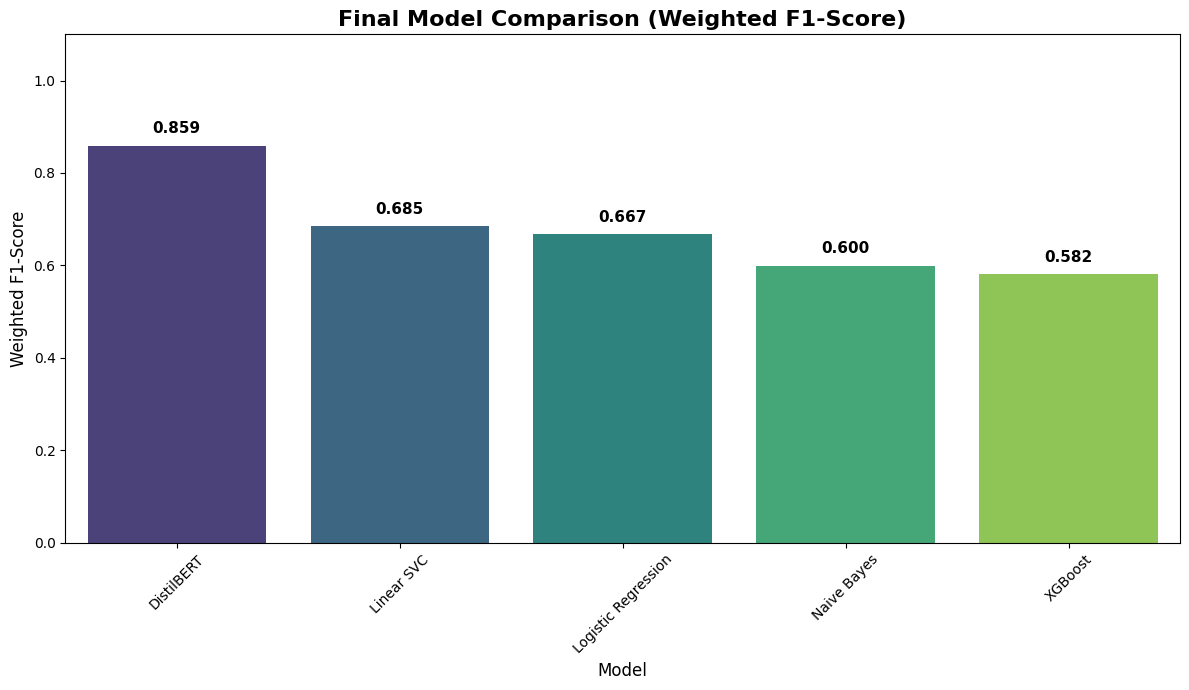
\includegraphics[width=0.9\linewidth]{compare-f1.png}
    \end{center}
\end{frame}

% ------------------------------------------------------------
\begin{frame}{Context-Free Sentiment Analysis}
    \begin{itemize}
        \item Removed video descriptions and classified only comments.
        \item Motivation: Instagram captions often non-informative.
        \item Performance largely unchanged; classical models slightly improved.
    \end{itemize}

    \begin{center}
        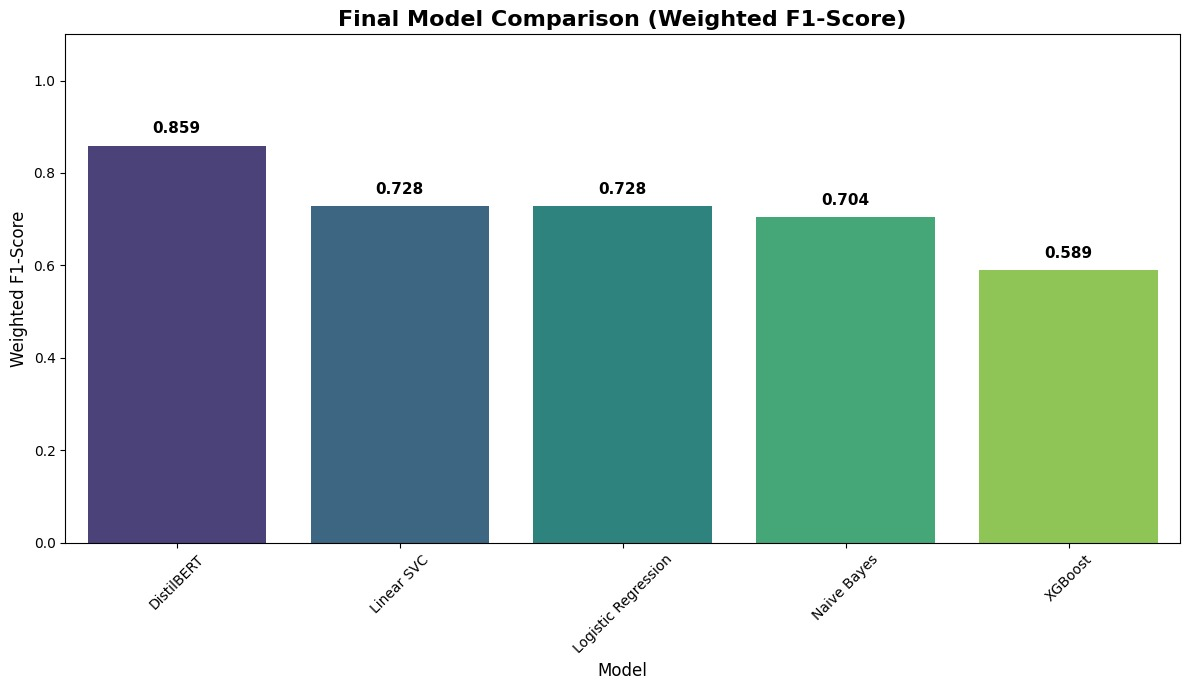
\includegraphics[width=0.9\linewidth]{context-free-f1.jpg}
    \end{center}
\end{frame}

% ------------------------------------------------------------
\begin{frame}{Conclusions}
    \begin{itemize}
        \item DistilBERT achieves the best overall performance.
        \item SVM is the most effective lightweight classical model.
        \item XGBoost performs poorly on sparse high-dimensional text.
        \item Entire pipeline feasible for real-world moderation tasks.
    \end{itemize}
\end{frame}

% ------------------------------------------------------------
\begin{frame}{Future Work}
    \begin{itemize}
        \item Insta-specific domain pretraining.
        \item Emoji-aware tokenisation.
        \item Multimodal (text + image) sentiment modelling.
        \item Continual learning for evolving slang.
    \end{itemize}
\end{frame}

% ------------------------------------------------------------
\end{document}
